

\section{Face Classification}

\label{sec:classification}
%We traverse each face in the intersection-free meshes, and classify which one belongs to the final mesh. Classification is done by evaluating the indicator vector $\bm{\Lambda}$ of each face. The basic idea of our classification method is to utilize the space coherence of face indicator vectors to share the classification results among neighboring faces. Also, because we store the neighborhood information in the edges which intersect other meshes, the search space of point-in-polyhedron test is limited to only a few faces. It makes the indicator computation very fast. Finally, by using P-reps, our classification method is exact can deal with any degenerate cases.

We traverse each face of the intersection-free meshes, and determine which belong to the final mesh. The faces are classified by evaluating the indicator vector $\bm{\Lambda}$ of each face. Our classification method utilizes the space coherence of the face indicator vectors to share the classification results among neighboring faces. Because we store the neighborhood information in the edges which intersect other meshes, the search space of the point-in-polyhedron test is limited. Hence, the indicator computation is very fast. Finally, because P-reps are used, our classification method is exact, and can deal with any degenerate cases.


%The space coherence of indicator vectors means neighboring faces may have the same indicator vector, or most components of indicator vectors. Therefore, we start from a seed face $\bm{s}_0$ with its indicator vector $\bm{\Lambda}(\bm{s}_0)$ known, and propagate to other faces in a flood-filling manner. The trace of indicator propagation is:

The space coherence of indicator vectors means that neighboring faces may have the same indicator vector, or most of the components of the indicator vectors. Therefore, we start from a seed face $\bm{s}_0$ with a known indicator vector $\bm{\Lambda}(\bm{s}_0)$, and propagate the indicator to other faces in a flood-filling manner. The trace of the indicator propagation is:

\begin{equation}
\label{eq:trace}
\bm{s}_0\to \bm{s}_1\to \bm{s}_2\to \bm{s}_3\to ...
\end{equation}


Intersection-free meshes facilitate this process by accelerating the indicator propagation. From adjacent faces $\bm{s}_1$ and $\bm{s}_2$, it is straightforward to determine whether $\bm{\Lambda}(\bm{s}_1)$ and $\bm{\Lambda}(\bm{s}_2)$ are different. The two indicator vectors are the same unless the shared edge $\bm{e}_{12}$ lies on the boundary of another mesh. In that cases, neighborhood information, say, $\bm{\mathcal{N}}(\bm{e}_{12}) = \{\mathcal{N}_k\}$, is stored on $\bm{e}_{12}$. Here we use $\bm{\mathcal{N}}$ to indicate that the edge may have more than one neighborhood (see \S\ref{sec:refine}). The neighborhood information indicates which components of the indicator vector differ between $\bm{s}_1$ and $\bm{s}_2$. If there is neighborhood information from mesh $M_x$, the $x^{th}$ indicators $\lambda_x(\bm{s}_1)$ and $\lambda_x(\bm{s}_2)$ differ, and can be computed efficiently and exactly with respect to that neighborhood. We outline our classification method in Algorithm \ref{code:floodfill}.

%Intersection-free meshes facilitate this process by accelerating the indicator propagation. From adjacent faces s1 and s2, it is straightforward to determine whether

\begin{algorithm}
\caption{Fast Face Classification}
\label{code:floodfill}
\textbf{Input: } Intersection-free hybrid meshes, boolean function $f$

\textbf{Output: } Classification $f(\bm{\Lambda}(\bm{s}_i))$ for all faces $\bm{s}_i$


\begin{algorithmic}[1]
\State Select a proper seed face $\bm{s}_0$
\State Compute the seed indicator vector $\boldsymbol{\Lambda}(\bm{s}_0)$
\State \Call{propagate} { $\bm{s}_0$ , $\boldsymbol{\Lambda}(\bm{s}_0)$}
\State
\Function{propagate}{ $\bm{s}$ , $\boldsymbol{\Lambda}(\bm{s})$}
    \State Compute $f(\boldsymbol{\Lambda}(\bm{s}))$
    \For {each neighboring face $\bm{s}_{s, i}$}
        \If {$\bm{s}_i$ has been classified}
            \State continue
        \EndIf
        \If {there are PBI-reps ${\bm{\mathcal{I}}}_k$ on $\bm{e}(\bm{s}_{s, i}, s)$}
            \State compute $\boldsymbol{\Lambda}(\bm{s}_{s, i})$ by $\boldsymbol{\Lambda}(\bm{s})$ and ${\bm{\mathcal{I}}}_k$
            \State \Call{propagate} { $\bm{s}_{s, i}$ , $\boldsymbol{\Lambda}(\bm{s}_{s, i})$}
        \Else
            \State \Call{propagate} { $\bm{s}_{s, i}$ , $\boldsymbol{\Lambda}(\bm{s})$}
        \EndIf
    \EndFor
\EndFunction
\end{algorithmic}
\end{algorithm}


\subsection{Indicator Propagation}
\label{sec:propagation}


%Meshes consist of vertices, edges and faces. Classification is required to perform on the face level. However, polyhedron-in-out test is performed based on points. Gaps exist between the them. Conventionally, face barycenter is used to compute the indicator of the whole face. This is because in intersection-free meshes, face is classified as a whole, and every face inner point will have the same indicator as the face's. However, the computation of inner point coordinates requires geometry construction, which introduces errors without exact arithmetic. Therefore, we use the face (or subface) vertices instead, whose exact representations are known, for indicator computation.

Meshes consist of vertices, edges and faces. It is necessary to perform classification at the face level. However, polyhedron-in-out tests are performed on points, where gaps exist between them. Conventionally, the face barycenter is used to compute the indicator of the whole face because in intersection-free meshes, the face is classified as a whole, and every inner point of the face will have the same indicator as the whole face. However, the computation of inner point coordinates requires geometric constructions, which introduce errors unless exact arithmetic can be used. Therefore, we use the face (or subface) vertices instead, the exact representations of which are known, for indicator computation.

\begin{wrapfigure}{r}[0in]{0in}
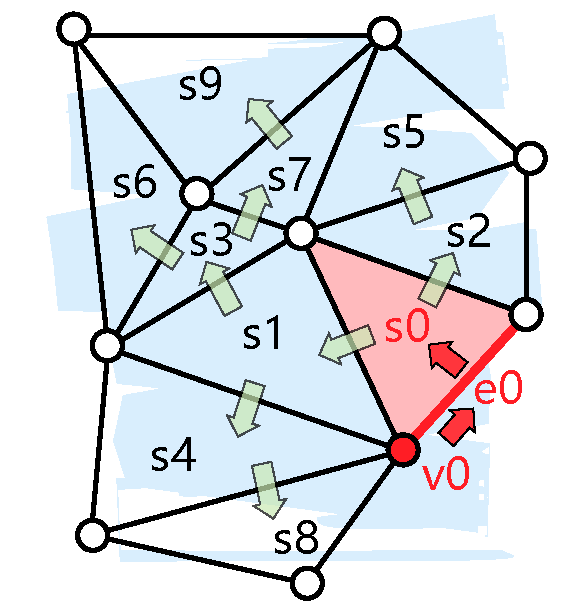
\includegraphics[width=1.3 in]{propagate}
\end{wrapfigure}


%However, there are two gaps between face indicator and face vertex indicator. First, the indicator of vertex does not always equal to indicator of face. Second, face indicator has two extra classes in $on$ case---$same$ and $oppo$, because the face has its orientation.


\begin{figure}[t]
\centering
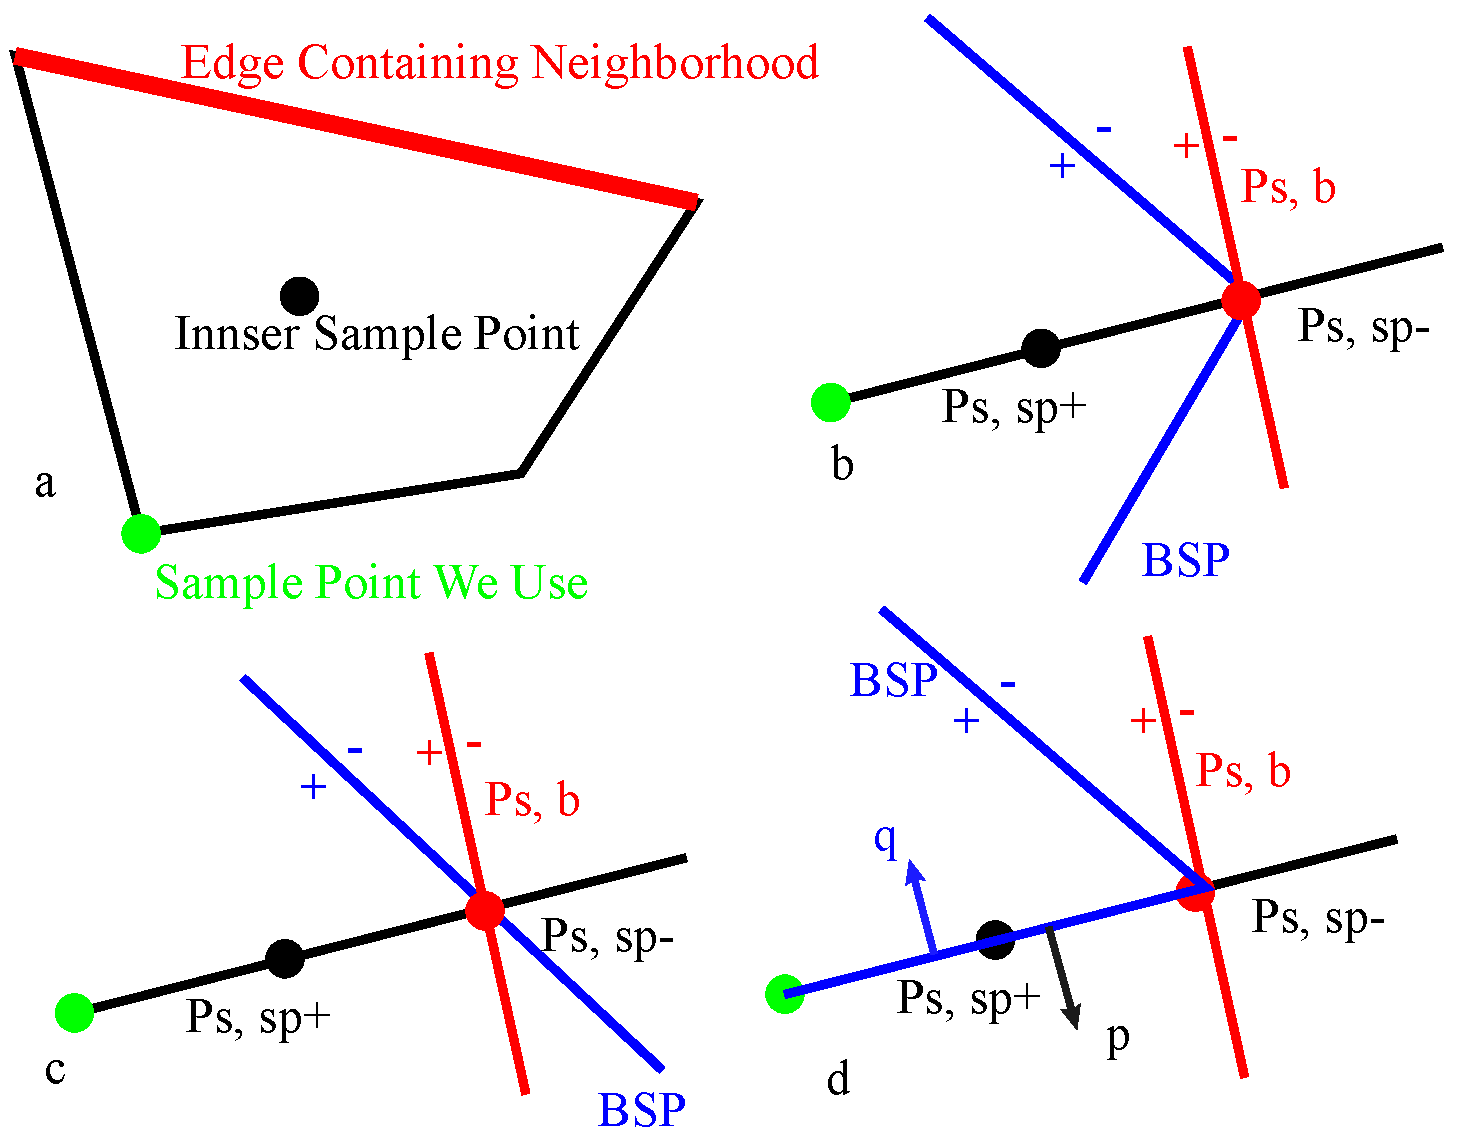
\includegraphics[width=3in]{bsps}
\caption{a) Because the inner sample point includes geometric constructions, we choose the face vertex (orange) instead to compute the face indicator. b-d) Different types of classification. The simple structure of the neighborhood BSP guarantees the same classification result for all of the points on $\bm{p}_{\bm{s}, sp}^+$. In d), the classification result is $on$ so it is necessary to determine the orientation from the normal of the BSP splitting plane $q$ and the face normal $p$. In this cases, the indicator should be $oppo$ because $p$ and $q$ are opposite.}
% a) Because the
\label{fig:bsps}
\end{figure}


However, there are two discrepancies between the face and face vertex indicators. First, the vertex indicator is not always equal to the face indicator. Second, the face indicator has two extra classes in the $on$ case��$same$ and $oppo$��because the face has an orientation.

%To overcome the gaps, we rewrite our indicator trace (\ref{eq:trace}) in finer granularity. In the beginning, we start from a seed vertex $\bm{v}_0$ on seed face $\bm{s}_0$. We assume indicator vector $\bm{\Lambda}(\bm{v}_0)$ is known. Then we use $\bm{\Lambda}(\bm{v}_0)$ to compute $\bm{\Lambda}(\bm{s}_0)$. In addition, we add an optional edge layer into the trace. Then it changes to:

To deal with these discrepancies, the indicator trace (\ref{eq:trace}) is modified for finer granularity. We start from a seed vertex $\bm{v}_0$ on a seed face $\bm{s}_0$. We assume that the indicator vector $\bm{\Lambda}(\bm{v}_0)$ is known. Then we use $\bm{\Lambda}(\bm{v}_0)$ to compute $\bm{\Lambda}(\bm{s}_0)$. In addition, we add an optional edge layer into the trace:

\begin{equation}
\bm{v}_0\to \bm{e}_0\to \bm{s}_0\to (\bm{e}_1)\to \bm{s}_1\to (\bm{e}_2)\to \bm{s}_2\to ...,
\end{equation}
%where $\bm{v}$ and $\bm{e}$ are the vertex and edge, respectively. The bracket indicates that propagating to the edge is optional, because if the edge does not contain neighborhood information the indicators on the two side are the same and we do not need to propagate to the edge. We find that there are three kinds of basic operations in the trace: $\bm{v}_{\bm{e}}\to \bm{e}$, $\bm{e}_{\bm{s}}\to \bm{s}$ and $\bm{s}\to \bm{e}_{\bm{s}}$, where $\bm{v}_{\bm{e}}$ means the end point of $\bm{e}$, and $\bm{e}_{\bm{s}}$ means the edge of $\bm{s}$.
where $\bm{v}$ and $\bm{e}$ are the vertex and edge, respectively. The bracket indicates that propagating to the edge is optional, because if the edge does not contain neighborhood information the indicators on either side are the same, so we do not need to propagate to the edge. There are three basic operations in the trace: $\bm{v}_{\bm{e}}\to \bm{e}$, $\bm{e}_{\bm{s}}\to \bm{s}$ and $\bm{s}\to \bm{e}_{\bm{s}}$, where $\bm{v}_{\bm{e}}$ is the end point of $\bm{e}$, and $\bm{e}_{\bm{s}}$ is the edge of $\bm{s}$.

%Given the partial order $on \succ in$ and $on \succ out$, our key observation is that the following relation always stands for indicators within intersection-free meshes:
Given the partial orders $on \succ in$ and $on \succ out$, the following relationship is true for indicators within intersection-free meshes:

\begin{equation}
\label{eq:porder}
\lambda_k(\bm{v}_{\bm{e}_{\bm{s}}}) \succeq \lambda_k(\bm{e}_{\bm{s}}) \succeq \lambda_k(\bm{s}),
\end{equation}
where $\lambda_k(x)$ is the indicator of $x$ for a certain primitive $M_k$. This relationship can be inferred from the continuous space assumption and the definition of intersection-free mesh*. It indicates that when we perform $\bm{v}_{\bm{e}}\to \bm{e}$ and $\bm{e}_{\bm{s}}\to \bm{s}$, from a low-dimension to a high-dimension, we decide whether the $on$ indicator changes to $in$ or $out$, or remains $on$. When we perform $\bm{s}\to \bm{e}_{\bm{s}}$, we decide whether $in$ and $out$ indicators are changed to $on$. In addition, when considering the orientation of the face, we also need to determine whether the $on$ indicators change to $same$ or $oppo$ during the $\bm{e}_{\bm{s}}\to \bm{s}$ operation.

%where

\vspace{0.5em}
\noindent\textbf{$\bm{s\to \bm{e}_{\bm{s}}}$}~~~~ We need to determine which indicators change to $on$. We know that when $\lambda_k(\bm{e}_{\bm{s}})=on$, there will be neighborhood information related to mesh $M_k$ stored on $\bm{e}_{\bm{s}}$. Therefore, in this operation, we need to traverse all of the neighborhoods of $\bm{e}_{\bm{s}}$ and change the corresponding indicators to $on$.

%s


\vspace{0.5em}
\noindent\textbf{$\bm{\bm{e}_{\bm{s}}\to \bm{s}}$}~~~~From eq. \ref{eq:porder}, we know that if $\lambda_k(\bm{e}_{\bm{s}}) \neq on$, then $\lambda_k(\bm{e}_{\bm{s}})=\lambda_k(\bm{s})$. Conversely, when $\lambda_k(\bm{e}_{\bm{s}}) = on$, $\lambda_k(\bm{s})$ can be determined using neighborhood information related to $M_k$. The neighborhood of $M_k$ can be either a face or a set of faces from the mesh $M_k$.  We can build a trivial BSP \cite{thibault1987set} using these faces. The BSP can be used to compute $\lambda_k(\bm{s})$ if a point can be sampled from $\bm{s} \cap \bm{U}(\bm{e}_{\bm{s}})$, where $\bm{U}(\bm{e}_{\bm{s}})$ is the neighborhood space of $\bm{e}_{\bm{s}}$. Unfortunately, we cannot guarantee that such a point can be found with precise coordinates.

%
\vspace{0.5em}
\begin{wrapfigure}{r}[0in]{0in}
 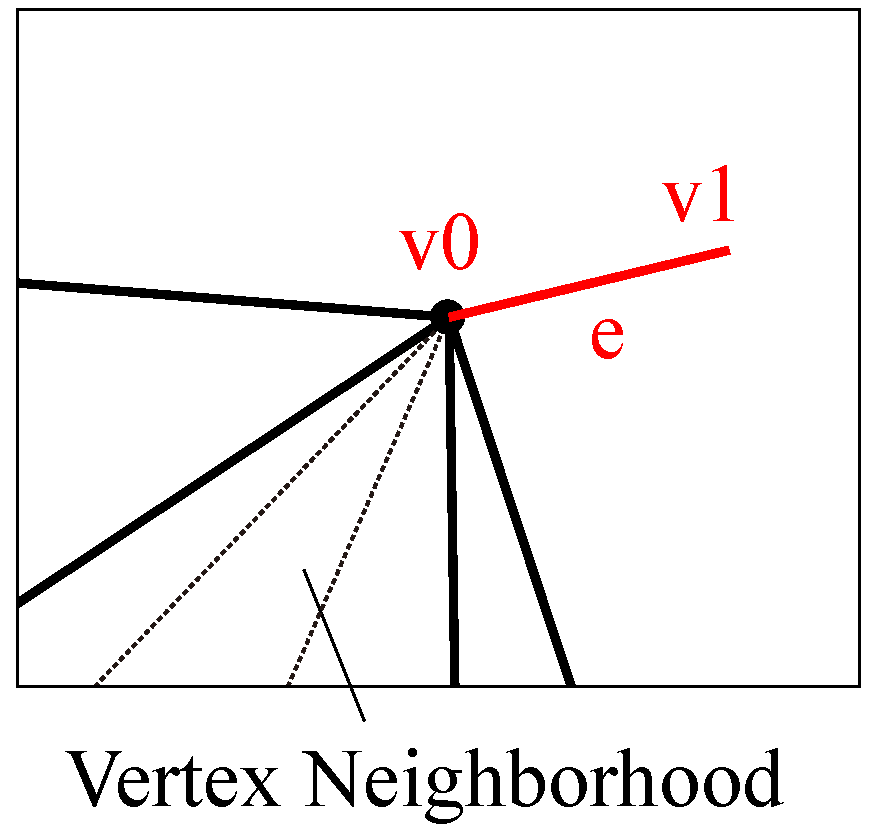
\includegraphics[width=1.3 in]{vneighbor}
\end{wrapfigure}
Our BSP is constructed from a single face, or a set of faces sharing the same edge. This BSP is sufficiently simple that the indicators $\lambda_k$ of all of the points on the half plane $\bm{p}_{\bm{s}, sp}^+$ are identical. Here $\bm{p}_{\bm{s}, sp}^+$ is half of the supporting plane of $\bm{s}$ that lies on the positive side of the bounding plane $\bm{p}_{\bm{s}, b}^{\bm{e}_{\bm{s}}}$ (Fig. \ref{fig:bsps}). Since $\bm{p}_{\bm{s}, sp}^+ \cap \bm{s} \neq \varnothing$, we can compute $\lambda_k(\bm{s})$ by determining $\lambda_k(\bm{v}_x, \bm{v}_x \in \bm{p}_{\bm{s}, sp}^+)$. For polygons, at least one corner point lies on $\bm{p}_{\bm{s}, sp}^+$, and the exact coordinates of the corner point are known. That corner point is used as $\bm{v}_x$. In addition, we assign each BSP splitting plane a normal from the normal of the triangle it contains, from which we can decide the orientation ($same$ or $oppo$) when $\lambda_k(\bm{s})=on$.

%Our BSP is constructed from a single face, or a set of faces sharing the same edge. This BSP is sufficiently simple that the indicators

\noindent\textbf{$\bm{\bm{v}_{\bm{e}}\to e}$}~~~~If $\lambda_k(\bm{v}_{\bm{e}})=on$, we first check whether $\lambda_k(\bm{e}) = on$, by checking whether there is neighborhood information related to $M_k$ on $\bm{e}$. If not, we need to find where $\bm{v}_{\bm{e}}$ lies on $M_k$. This is straightforward because the intersection-free meshes contain geometric connectivity information. We can consider the connectivity information as the vertex version of neighborhood information, and the same BSP-based classification method is used in ${\bm{e}_{\bm{s}}\to \bm{s}}$ can be used to determine the high dimension indicator $\lambda_k(\bm{e})$. We use the other end point $\bm{v}'_{\bm{e}}$ as the sample point for the BSP classification.

%ve


\subsection{Acceleration by Caching}
\label{sec:acc}
%If the CSG tree is large with hundreds of primitive nodes, computing $\lambda_f(\bm{s}_i)$ from $\boldsymbol{\Lambda}(\bm{s}_i)$ for every face $\bm{s}_i$ can be costly. Thanks to the indicator space coherence, we can save the computation time by caching the evaluation result during flood-filling.

If the CSG tree is large, with hundreds of primitive nodes, computing $\lambda_f(\bm{s}_i)$ from $\boldsymbol{\Lambda}(\bm{s}_i)$ for every face ($\bm{s}_i$) can be costly. However, using indicator space coherence, we can reduce the computation time by caching the evaluation results during flood-filling.

%The basic cache strategy is to cache final result, that is, the value of $\lambda_f(\bm{s}_i)$. We know indicator vector will not change if there is no intersection edge during propagation. That means the final classification $\lambda_f(\bm{s}_i)$ will not change, too. Thus, those faces sharing the same indicator vector can be classified as a whole.

The basic caching strategy is to cache the final result, that is, the value of $\lambda_f(\bm{s}_i)$. We know that the indicator vector will not change if there is no intersection edge encountered during propagation. Therefore, the final classification $\lambda_f(\bm{s}_i)$ will not change either. Thus, faces which share the same indicator vector can be classified as a set.

%Also, we can perform intermediate results cache. We noticed that the boolean expression can be simplified if some components of $\bm{\Lambda}(\bm{s}_i)$ is fixed. For example, assume we have a boolean expression $f = M_1\cup (M_2\cap M_3-M_4)$. Given the values of two indicators $\lambda_1(\bm{s}_i)=out$, $\lambda_2(\bm{s}_i)=in$, the expression can be rewritten as $f(\lambda_1=out, \lambda_2=in)=out\cup (in\cap M_3-M_4)$. Using the combination rules we can simplify the expression as $f(\lambda_1=out, \lambda_2=in)=P_3-P_4$. Because for a large CSG, a certain mesh often intersects with only a few other meshes $\Theta= \{M_{n_1}, M_{n_2}, \cdots, M_{n_x}\}$. That means all the faces in this mesh has the same indicators against $M_{i} \notin \Theta(M_k)$. Therefore, we can first determine these fixed indicators and simplify the boolean function, and then use simplified one to compute the final indicator for each faces in this mesh.

We can also perform an intermediate results cache. The boolean expression can be simplified if some components of $\bm{\Lambda}(\bm{s}_i)$) are fixed. For example, assume we have a boolean expression $f = M_1\cup (M_2\cap M_3-M_4)$. Given the values of two indicators $\lambda_1(\bm{s}_i)=out$, $\lambda_2(\bm{s}_i)=in$, the expression can be rewritten as $f(\lambda_1=out, \lambda_2=in)=out\cup (in\cap M_3-M_4)$. Using the combination rules, we can simplify the expression to $f(\lambda_1=out, \lambda_2=in)=M_3-M_4$. In a large CSG, a given mesh often intersects with only a few other meshes $\Theta= \{M_{n_1}, M_{n_2}, \cdots, M_{n_x}\}$. Thus, all of the faces in this mesh have the same indicators for $M_{i} \notin \Theta(M_k)$. Therefore, if we can determine the fixed indicators and simplify the boolean function, then we compute the final indicator for each face in this mesh.


\iffalse
\subsection{Tessellating on Classification}
We find for a CSG with many meshes, a large percentage of intersections are invalid (see \S\ref{sec:degenerate} for 'invalid'). Tessellation according to these invalid intersections is not necessary. To avoid unnecessary tessellation, we can give an early prediction of which intersections are invalid by intersections information of faces, but have to embed the tessellation stage into the classification stage, which we call it 'tessellating on classification'.

In most situations, a certain faces $\bm{s}$ only intersect with a few other meshes $\Theta(\bm{s})$. We can use the same cache strategy in \S\ref{sec:acc} to shrink the original CSG into a smaller one by the common indicators of $\{P_i\}\backslash\Theta(\bm{s})$, where $\{P_i\}$ means all the primitive meshes. After the shrinking, the primitive meshes of the CSG must be from $\Theta(\bm{s})$. If any mesh in $\Theta(\bm{s})$ does not appear in the shrinked CSG, it means the indicator of that mesh does not change the classification result, which in another word, intersections on $\bm{s}$ from that mesh are invalid and do not affect the classification of any subfaces of $\bm{s}$. If the shrinked CSG is trivial which does not contain any primitives, it means $\bm{s}$ does not need tessellation. In this way, we save the computation time, and simplify the topology of the final result mesh. Because we can only shrink the CSG for $\bm{s}$ when we classify it---before that the indicators of meshes from $\{P_i\}\backslash\Theta(\bm{s})$ are not known---we do not perform tessellation until we do the classification.
\fi
